\documentclass[10pt,twocolumn,letterpaper]{article}

\usepackage{../authorkit/cvpr}
\usepackage{times}
\usepackage{epsfig}
\usepackage{graphicx}
\usepackage{amsmath}
\usepackage{amssymb}

% Packages added by us
\usepackage{amsfonts}
\usepackage{mydefs}
\usepackage{algorithmic}
\usepackage{algorithm}

\usepackage[pagebackref=true,breaklinks=true,letterpaper=true,colorlinks,bookmarks=false]{hyperref}

% \cvprfinalcopy % *** Uncomment this line for the final submission

\def\cvprPaperID{****} % *** Enter the CVPR Paper ID here
\def\httilde{\mbox{\tt\raisebox{-.5ex}{\symbol{126}}}}

% Pages are numbered in submission mode, and unnumbered in camera-ready
\ifcvprfinal\pagestyle{empty}\fi
\begin{document}

%\title{Accelerating $\ell_1$-Minimization Using Many-Core CPUs/GPUs \\ and Application to Face Recognition
%\title{Efficient Parallelization of Sparse Representation for Face Recognition}
%\thanks{Corresponding author: . This work was partially supported by ARO MURI W911NF-06-1-0076.}}
\title{Efficient Parallelization of $\ell_1$-Minimization for Face Recognition
\thanks{Corresponding author: . This work was partially supported by ARO MURI W911NF-06-1-0076.}}

\author{First Author\\
Institution1\\
Institution1 address\\
{\tt\small firstauthor@i1.org}
% For a paper whose authors are all at the same institution,
% omit the following lines up until the closing ``}''.
% Additional authors and addresses can be added with ``\and'',
% just like the second author.
% To save space, use either the email address or home page, not both
\and
Second Author\\
Institution2\\
First line of institution2 address\\
{\small\url{http://www.author.org/~second}}
}

\maketitle

\begin{abstract}

\end{abstract}

\section{Introduction} 

%Motivate the paper by an overview about the scope and importance of $\ell_1$-minimization.
$\ell_1$-minimization is one of the most powerful tools to be added to the engineer's
toolbox in years.  It has strong theoretical motivation for both for use in recovering sparse
solutions to systems of linear equations, and has been shown to perform well even in the
presence of a combination of sparse and dense error.  Since solutions of linear systems
arise in practically every branch of engineering and there are very few application which
do {\em not} benefit from a robust error function, the applications are far to numerous to
itemize here.  
For many applications of $\ell_1$-minimization solving a system $b=Ax$, $A$ often has a
special structure that can be leveraged to compute portions of $A$ on the fly
as they are needed, speeding up perfomance of the minimization dramatically.
Unfortunately, there are many import applications where this does not hold true.
This paper targets applications where $\bb$ and $A$ contain
image data, and thus must be loaded every time they are used, as is the 
case for many problems in computer vision.
The techniques presented in this paper target these applications, as well
as others where the dictionary is dense and unstructured. $A$ must be loaded every time
it is used, and algorithm performance becomes highly dependent on memory bandwidth, rather
than arithmetic logic.

% Narrow focus for applications to Recognition Application
The primary motivating application for this paper is face recognition for access control applications.
Recently, advances in automatic face recognition have been made by re-casting
it as a sparse representation problem.  This core of this technique consists of
re-casting recognition as a sparse representation problem. This is done by  
stacking the test image into a vector $\bb$, stacking the training images for
all of the users into the columns of a matrix $A$, and solving the following
minimization problem:
\begin{equation}
\min_{\x, \e} \| \x \|_1 + \|\e\|_1 \quad \subj \quad \bb = A \x + \e.
\end{equation}
This optimization promotes a solution that is sparse both in $\x$ and $\e$. 
Sparsity in $\x$ arrises from the fact that only a subset of the training images (if any)
correspond to the user in the test image.  Sparsity in $\e$ arrises from the knowledge
that small occlusions in the test image will only corrupt a small subset of the pixels \cite{Wright2009-PAMI}.
The large coefficients in $\x$ will concentrate on the correct user, and can be used as the basis of a classifier.

For this idea to work, all of the images must be aligned. An iterative alignment
algorithm for this purpose was described as part of the \cite{Wagner2009-CVPR}, which was
the first paper to expand \cite{Wright2009-PAMI} into a functioning face recognition system.
This iterative alignment routine is based on repeatedly solving the following optimization problem:
\begin{equation}
\min_{\x, \e} \|\e\|_1 \quad \subj \quad \bb = A_k \x + \e.
\end{equation}
Where $A_k$ contains the training images for user $k$ as well as several vectors consisting of the
Jacobian of the test image $\bb$ with respect to the transformation parameters, and $\x$ contains
both the current representation coefficients, as well as an update to the transformation parameters.

\begin{figure}
\centering
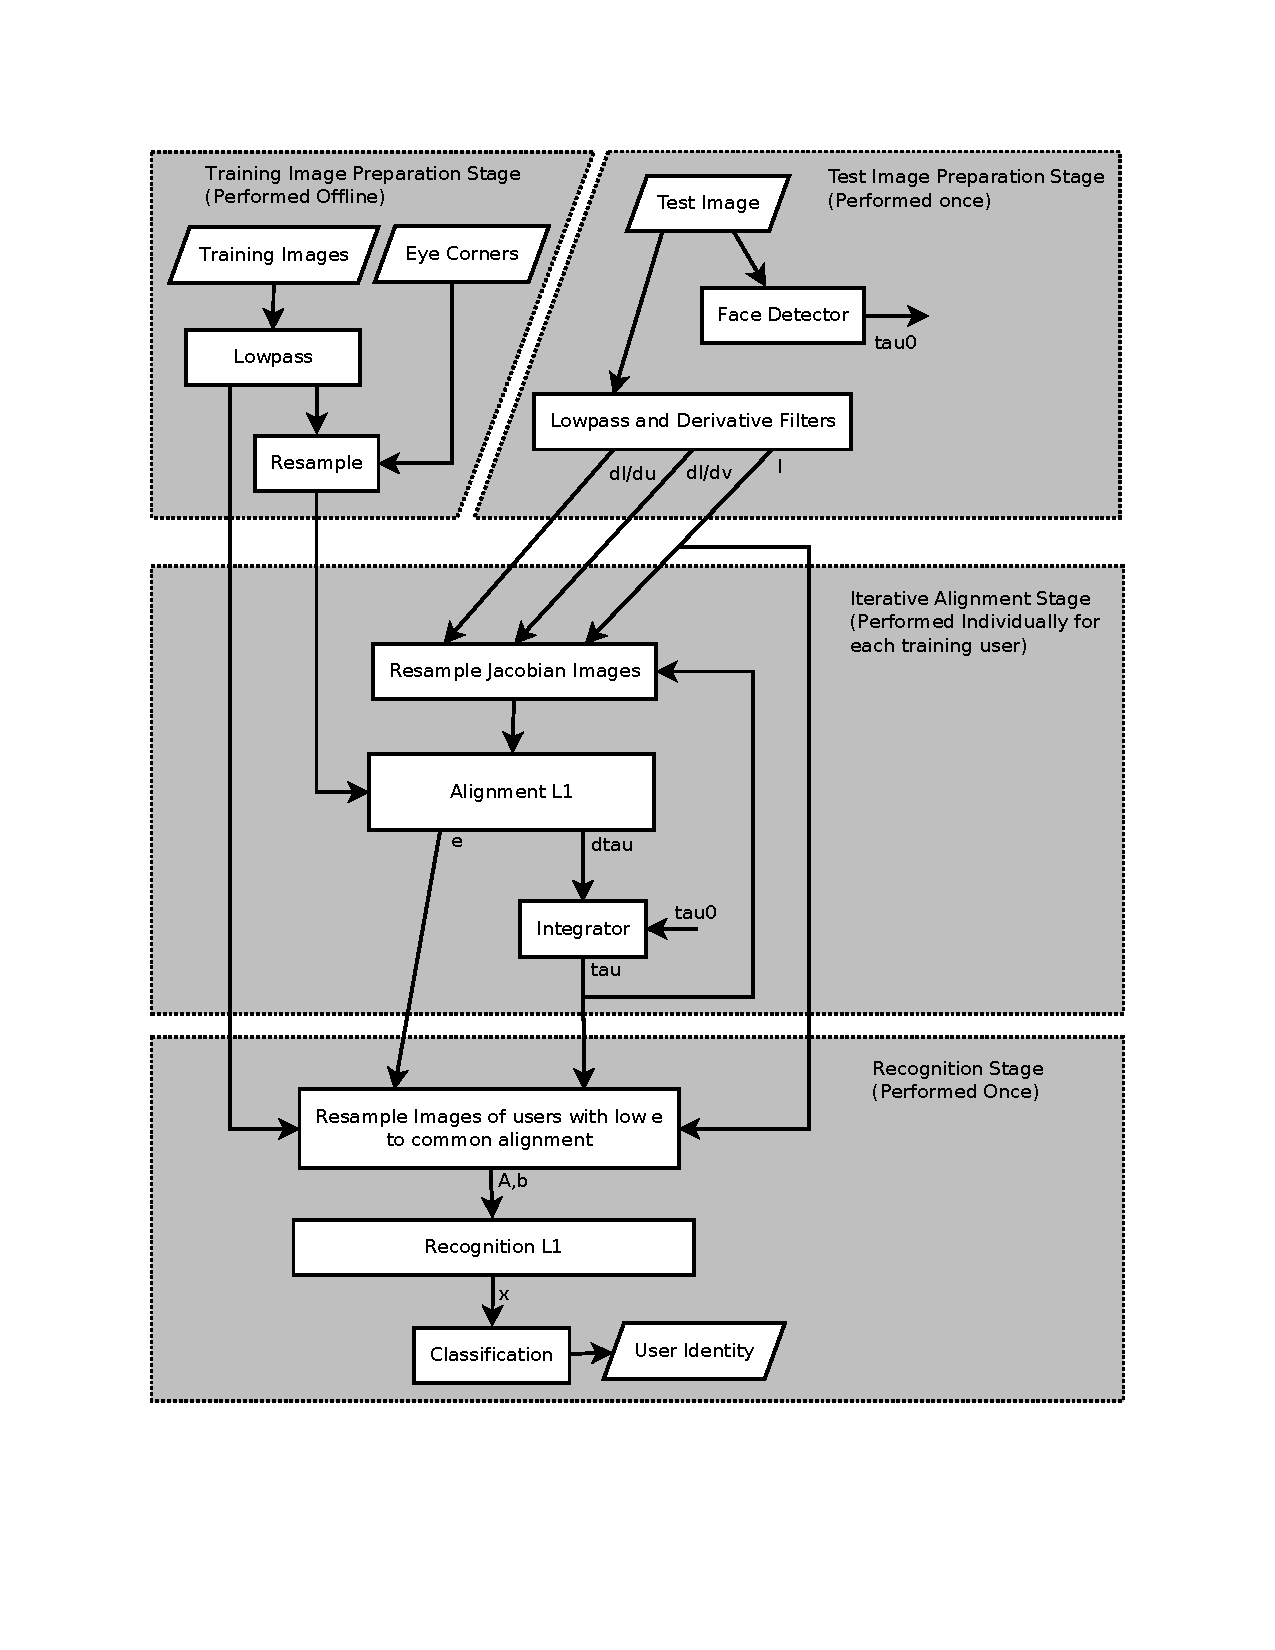
\includegraphics[width=3.5in]{figures/pipeline.pdf}
\caption{The Full Recognition Pipeline}
\label{fig:pipeline}
\end{figure}

\begin{figure}
\centering
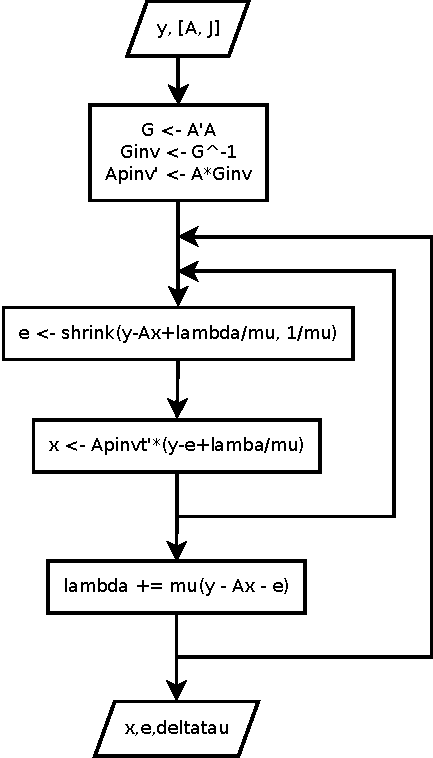
\includegraphics[width=3.5in]{figures/alignment_l1.pdf}
\caption{Alignment Stage L1 Solver}
\label{fig:alignment_l1}
\end{figure}

\subsection{Literature review}
%[Review the past parallel algorithms for $\ell_1$-minimization. Hopefully there aren't many]
%[Review the available different algorithms solving $\ell_1$-minimization and $\ell_0$-minimization, please refer to Allen's SIAM paper.
%[Zero in and justify why we choose ALM for our implementation.]

Standard solvers for $\ell_1$-minimization include orthogonal matching pursuit, basis pursuit and LASSO which cast the $\ell_1$-minimization as either a linear program or quadratic program.  

These methods can be accelerated by more contemporary methods such as gradient projection, homotopy, iterative shrinkage-thresholding, proximal gradient, and augmented lagrangian methods.  According to analysis of these five algorithms applied to face recognition, Yang et al have determined that Homotopy and the Augmented Lagrangian Multiplier methods (ALM) achieve the best recognition rates while maintaining a low computational cost.  A closer look at these two algorithms will show that while the Homotopy method will produce the exact solution, the algorithm structure and functions do not lend themselves parallelization well.  
On the other hand, while the ALM finds an approximate solution, its computation mainly consists of matrix-vector operations, which lends itself to parallelization.

Past work in parallelizing $\ell_1$-minimization has been limited.  In 2009, Murphy at UCB implemented the L1-Spirit algorithm on Nvidia GPUs for MRI reconstruction and in 2009 Borghi at UCLA developed a proximal point algorithm using Moreau-Yosida regularization, which is special form of the $\ell_1$-minimization based on proximal gradient.  

\subsection{Contributions of the paper}

\section{Augmented Lagrangian Multiplier Algorithm}

In this section, we describe the general version ALM algorithm and then describe how it can be adapted to solve our problem.

The augmented lagrange multiplier (ALM) method utilizes a popular class of convex techniques, the lagrange multiplier, solving the problem:
\begin{equation}
F(x) = f(x) + \lambda g(x).
\end{equation}
which can be formulated as an augmented Lagrange function given by
\begin{equation}
L_u(x,y) = \|x\|_1 + <\y, b - A\x - \e> + \frac{\mu}2 \| b-A\x-\e \|_2^2
\end{equation}

where $\mu > 0$ is a constant that penalizes infeasibility and $y$ is a vector of lagrange multipliers.

For an optimal $y*$ which satisfies the second-order sufficiency conditions, for a sufficiently large $mu$, it can be shown that
\begin{equation}
x* = \arg min L_u(x,y*)
\end{equation}

However, because $y*$ is generally unknown, ALM methods simultaneously estimate the optimal solution and Lagrange multipliers iteratively in the following procedure.

We also need to define the following soft-thresholding operator for a
scalar $x$ and a scalar $\alpha \geq 0$:
\begin{equation}
\textup{shrink}(x,\alpha) = \textup{sign}(x)\cdot \max \{|x| - \alpha, 0\},
\end{equation}
In practice, this operator will be applied elementwise to a vector $\x$ with a single $\lambda$,
and will be notated as $\textup{shrink}(\x,\alpha)$.

We summarize the entire ALM
algorithm as Algorithm~\ref{alg:alm}, where $\gamma$ denotes the largest eigenvalue of the matrix $A^TA$. For the choice of parameter $\mu$, we take the same strategy as
in \cite{YangJ2009-pp} and set $\mu_0 = 2m / \|\bb\|_1$. We set $\rho=1.5$.
\begin{algorithm}[h]
\caption{\bf (Augmented Lagrange Multiplier Method FIX)}
\begin{algorithmic}[1]
\STATE {\bf Input:} $\bb \in \Re^m$, $A \in \Re^{m \times n}$,
$\x_1 = \mathbf{0}$, $\blamda_1 = \mathbf{0}$.
\WHILE{not converged ($k = 1,2,\ldots$)}
\STATE $t_{1} \leftarrow 1, z_{1} \leftarrow \x_{k}, \u_{1} \leftarrow \x_{k}$;
\WHILE{not converged ($l = 1,2,\ldots$)}
\STATE $\e_{l+1} \leftarrow \textup{shrink}\left(\bb - A\x_l + \frac{\blamda_k}{\mu_k}, \frac{1}{\mu_k}\right)$;
\STATE $\x_{l+1} \leftarrow (A^\dagger)^T \left(\bb - \e_{l+1} + \frac{\blamda_k}{\mu_k} \right) $;
\ENDWHILE
\STATE $\blamda_{k+1} \leftarrow \blamda_k + \mu (\bb - A\x_{k+1} - \e_{k+1})$;
\STATE $\mu_{k+1} \leftarrow \rho\mu_k$;
\ENDWHILE \STATE
{\bf Output:} $\x^* \leftarrow \x_k, \e^* \leftarrow \e_k$.
\end{algorithmic}
\label{alg:alm}
\end{algorithm}

%In order to solve the alignment stage before recognition, we consider the $l_1$ problem: 
%\begin{equation} 
%\min_{\x, \e} \|\e\|_1 \quad \subj \quad \bb = A \x + \e.
%\end{equation}
%which is solved in a similar fashion.

% A note on alignment l1...
% With a reshuffling of the order of operations and a change of the termination
% condition, the inner loop takes the form of two matrix-vector multiplications
% and a sequence of vector-vector operations.

In order to adapt the general algorithm to face alignment and recognition, we formulated the 
$\ell_1$-minimization problem as ___ as described in [book].

\subsection{Alignment Stage L1 Computational Complexity} Any discussion of the speed of an
algorithm should discuss the comutational complexity of the algorithm.  For the
ALM algorithms considered in this paper, this is rather simple.  The
Matrix-vector computions are $O(mn)$, and the vector-vector operations are
$O(m)$, in terms of both computation cost and memory-bandwidth.  Since A is
very tall, the computation of $A^\dagger$, the pseudoinverse of $A$, is best
computed via $A^\dagger = (A^TA)^{-1} A^T$.  The complexity of computing $G =
A^T A$ is $O(nnm)$.  $G$ is sufficiently small that it can be inverted via
Gauss-Jordan elimination, which has a complexity of $O(n^3)$.  The computation
of $A$ finishes with a matrix multiplication, with cost $O(n^2 m)$.
Fortunately, $A^\dagger$ only needs to be computed once per instance of the
$\ell_1$ minimization problem.

Therefore, for problems with large $n$, we expect the computation of the
pseudoinverse to dominate.  However, for the problem sizes needed in face
recognition problems, we find that the computation time is dominated by the
repeated computation of matrix-vector and matrix-matrix multiplications in the
inner loop.

\section{Hardware Parallelism} 
In this section we give a brief overview of the hardware architectures used
in this paper.

We feel it is most meaningful to compare hardware architectures on a per-board basis,
and in a typical hardware configuration.  GPU's are most commonly shipped with a single
GPU chip per PCI-express card.  
%For multicore CPU architectures, a typical workstation
%will consist of 

For CPU implementations, the benchmarks makes use of all of
the cores in as many cpu's are present.  For GPU implementations, the benchmark
makes the best use of the entire GPU chip (most GPU boards have a single GPU
chip).  Unless otherwise specified, all implementations utilize single
precision floating point datatypes.  

\subsection{CPU Hardware Parallelism} 
The baseline architecture for our experiments is a typical workstation,
with two quad-core Intel Nehalem E5530 processors clocked at 2.4 GHz.  Each
processor has its own memory interface, and is directly connected to half of
the RAM installed in the machine.  The amount of RAM installed exceeds the
amount used by the algorithms, and is not an important performance
consideration.  

Each core has a 32 KB L1 data cache and a 256 KB L2 cache. With Hyperthreading
enabled, each core can support two threads simultaneously.  For floating point
math, each core also has a vector unit capable of performing the same
arithmetic operation on four single precision floating point values
simultaneously.  \footnote{The core also has scalar floating point units, but
some compilers, notably gcc, generate code that uses the vector units
exclusively for floating point math.} 

There are thus two important levels of parallelism that need to be exploited to
use a modern cpu efficiently: core-level parallelism and vector-level
parallelism.  For the implementations discussed here, we will primarily use the
OpenMP programming model to express core-level parallelism.  Depending on the
section of the code, we will achieve vector-level parallelism implicitly
through either the auto-vectorization features of Intel's icc compiler, or
through the use of a highly optimized BLAS library (Intel's MKL).

Each processor has 8MB of L3 cache that is shared by all four cores.  Overall,
this means the algorithm has approximately 16MB of on-chip cache available.
For the low resolution images used in sparse representation based face
recognition, this is enough cache to hold over 800 image-sized variables,
meaning that for small data sets it is possible to run completely using on-chip
cache.

\subsection{GPU Hardware Parallelism}
%High-level description of GPU parallelism, i.e.

The ALM algorithm requires many matrix-vector operations, this gives manycore processors such as GPUs a computational advantage for large problem sizes.  GPUs are comprised of several streaming multiprocessors (SMP) (16 for the Nvidia Fermi) which each contain 32 floating-point units.  Each SMP contains its own L1-cache and shared memory and all SMPs share a common L2-cache.  The GPU executes programs as SIMT (Single Instruction Multiple Threads) in groups of 32 threads called warps.  These warps are then grouped into higher levels called thread blocks and grids. The GPU contains an inverted memory hierarchy so that the L1 cache stays close to the cores, providing the increase in performance and a computational advantage over CPUs.  Unlike normal CPUs, the Nvidia Fermi has 768 kb of L1 cache/shared memory and 768kb of L2 cache.  This increase in performance doesn't come for free.  Because the GPU has it's own memory system, any data the GPU uses must be transferred from RAM to the GPU over PCI-Express, which has limited bandwidth.  However, the cost of these transfers are amortized by doing large amounts of computation at once, requiring code to be run completely on the GPU.  

The GPU can be analogous to a multi-core CPU processor, except with more sophisticated vector processing hardware.  Each thread block is a virtualized multiprocessor, which each thread as a virtualized scalar processor.  All of these differences allow GPUs to perform intensive calculations such as matrix-vector operations at much faster rates than CPUs. 


% This section is Drew's
\section{Iterative Alignment Stage Implementation}

\subsection{Iterative Alignment on the CPU}
%\subsection{Tuning the GEMV operation}
%When matrix-vector operations are called sequentially on the same data,
%the operation can be blocked so that each thread operates on the same block of data for each operation.
%For Single threaded MKL sgemv, Code took          0.0335823 msec per instance to run!
%For Automatic multi-threaded MKL sgemv, Code took 0.008179 msec per instance to run!
%For Manually multi-threaded MKL sgemv, Code took  0.0061276 msec per instance to run!

%\subsection{Tuning the Soft-Thresholding Operator}
%...Make sure there are no branches
%...Make sure there are no function calls
%...Make sure the loop gets automatically vectorized
%...Block the computation into work for different cpu cores
\subsection{Iterative Alignment on the GPU}
% Describingn the sequence of GPU implementations Drew has tried...

\subsection{Benchmark on Real Face Data}

\begin{figure}
\centering
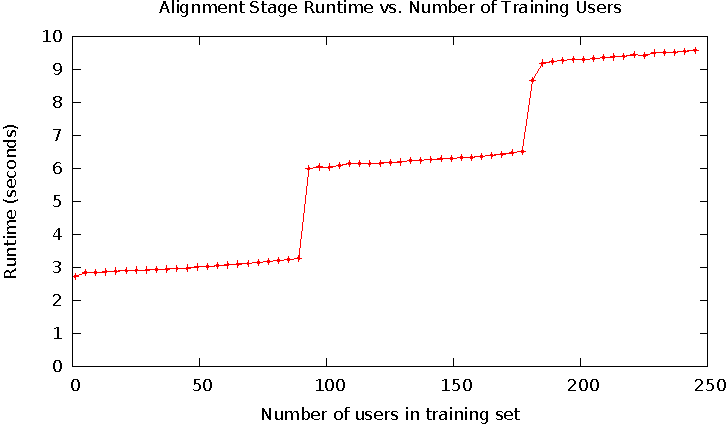
\includegraphics[width=3.5in]{figures/runtime_graph.pdf}
\caption{GPU Alignment Stage Time vs. Size of Database}
\label{fig:alignment_runtime}
\end{figure}

\section{Recognition Stage Implementation}
% This section is Victor's 

%The ALM algorithm requires many matrix-vector operations, this gives manycore
%processors such as GPUs a computational advantage for large problem sizes.
%GPUs are comprised of several streaming multiprocessors, which contain 32
%floating-point units.  The GPU executes programs as SIMT (Single Instruction
%Multiple Threads) in groups of 32 threads called warps.  These warps are then
%grouped into higher levels called thread blocks and grids.  The improvement in
%speed comes from the memory structure of the GPU.   The GPU contains an
%inverted memory hierarchy so that the L1 cache stays close to the cores,
%providing the increase in performance.  It essentially turns the GPU from being
%memory-limited to computational-limited.  GPU memory also differs from CPU
%memory in that it requires data transfers over PCI-Express.  The cost of these
%transfers are amortized by doing large amounts of computation at once,
%requiring code to be run completely on the GPU.  The GPU can be analogous to a
%multi-core CPU processor, except with more sophisticated vector processing
%hardware.  Each streaming multiprocessor is analogous to a single CPU except
%that it can run multiple threads simultaneously.  All of these differences
%allow GPUs to perform intensive calculations such as matrix-vector operations
%at much faster rates than CPUs.

% In the followingn 2 sections, just describe implementations; single number
% benchmarks and microbenchmarks are ok, but save big graphs for experiments
% section.

\subsection{ GPU Implementation}
The GPU ALM algorithm is written in CUDA and utilizes the CUBLAS libraries.
CUBLAS are the BLAS libraries consisting of all single precision BLAS calls
which are provided by Nvidia and are optimized for GPU performance. In
addition, we coded kernel (GPU) methods for vector-vector operations to replace
operations that would have taken multiple BLAS calls. Because data transfer from the RAM to GPU suffers bandwidth limitations, we designed our implementation to transfer the A matrix and measurement vector at once.  The algorithm is similar
to the CPU algorithm except that we had to parallelize the code at an
additional level. The CPU portion of the code serves as the conductor, making
calls to GPU functions and directing the flow of the code while the GPU keeps all of the data and runs the computation.

\subsection{Benchmark on Synthetic Data}

To construct the benchmark for synthetic data, we first created an $m \times n$
matrix $A$ with entries $\pm 1$ each with a $50\%$ chance.  Then we created a
sparse vector $\x_0$ with $10\%$ nonzero random entries.  We also created a
sparse vector $y_k$ with the same number of non-zero entries as $\x$.  Let
$\y_0 = A \x_0 + \y_k$.  We timed the time taken for the ALM algorithm using
$\y_0$, $A$, and other inputs.  The other inputs included, maximum number of
inner/outer loop iterations, and inner/outer loop tolerance level.

To simply the benchmark, we cap the number of inner iterations at 50 and outer iterations
at 5000 and run the algorithm to convergence.  CPU code was run on an Intel
Dual Socket Quad Core with 8 gigs of DDR3 RAM.  GPU code was run on a GTX480 We
ran the A matrix with different ratios between m:n from 10:1:5 for m:2000:25:8000 with an x vector of 10 percent sparsity.  Tolerance levels were
empirically seen to allow best performance with the inner loop tolerance set at
one order of magnitude lower than the outer loop tolerance.

Results were plotted as total size of A and A'A vs Gb/s and size of A vs time
elapsed to run a single $\ell_1$ solver.

\begin{figure*}
\centering
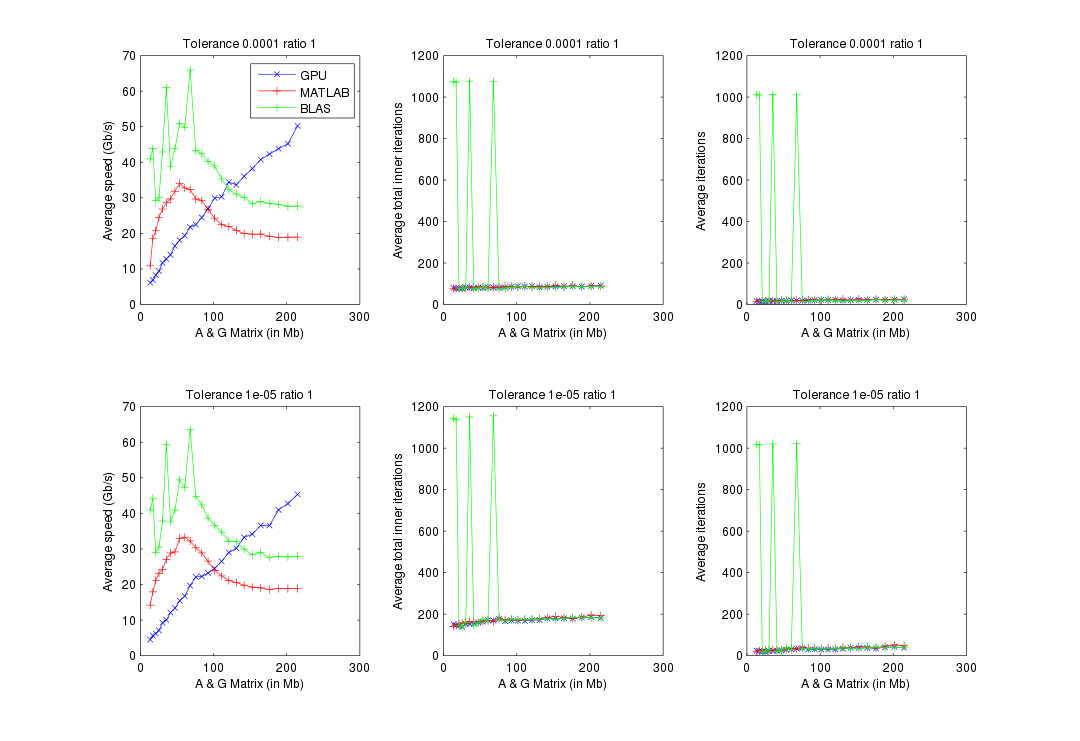
\includegraphics[width=3.5in]{figures/PALM_benchmark_ratio_1.png}
\caption{This is where the caption goes.}
\label{fig:uniqueidentifierforthisimage}
\end{figure*}

As the dimensions of $A$ increase, so does the significance of the size of
$A^TA$.  Until the $A$ and $A^TA$ reach ???? Mb (SHOULD BE MB?), the CPU version runs faster
than the GPU.  

\section{Full Pipeline Benchmarks}

\section{Conclusion}

{\small
\bibliographystyle{../authorkit/ieee}
\bibliography{faces}
}

\end{document}
